\section{Проектування системи відстеження напрямку погляду}
\subsection{Розробка вимог до програмної системи}
\subsubsection{Галузь застосування}
Данний продукт може бути використаний медичними програмами (контролювання курсору миші поглядом), та в цілях сбору пасивної інформації про точку погляду користувача персонального комп'ютера.

\subsubsection{Функціональні вимоги}
Список функціональних вимог до системи:
\begin{enumerate}[label={\arabic*)}]
	\item система повинна мати можливість налаштування під навколишнє середовище (тип веб-камери, положення мониторів комп'ютера);
	\item система повинна визначати точку погляду користувача;
	\item система повинна переміщувати курсор за допомогою погляду;
	\item система повинна працівати з однією веб-камерою.  
\end{enumerate}

\subsubsection{Нефункціональні вимоги}
Список нефункціональних вимог до системи:
\begin{enumerate}[label={\arabic*)}]
	\item похибка визначення точки погляду не більше ніж 4 см.;
	\item система повинна бути платформонезалежною та підтримувати такі операційні системи, як Debian, Windows, macOS;
	\item система повинна бути не вимогливою до веб-камери та комп'ютеру.
\end{enumerate}

\subsection{Архітектура програмної системи}
Для реалізації системи була обрана однорівнева архітектура \textit{(standalone application)}.

Однорівнева архітектура була обрана через те, що для відстеження напрямку погляду необхідно обробляти відеопоток, що потребуватиме надсилання великого об'єму данних на сервер.
Цей спосіб буде потребувати багато ресурсів сервера та може стати проблемою для конфіденціальності користувача.  

\subsubsection{Діаграма компонентів}
На рисунку~\ref{fig:component} зображена діаграма компонентів системи.

\begin{figure}[H]
	\centering
	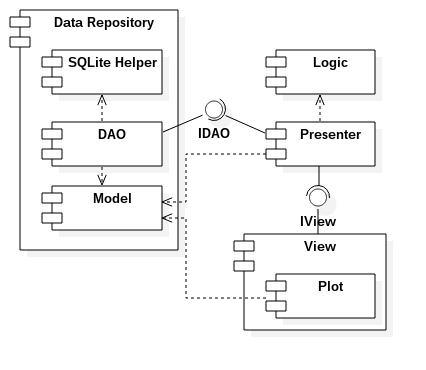
\includegraphics{uml_component}
	\caption{UML-діаграма компонентів}
	\label{fig:component}
\end{figure} 

Головними компонентами є:
\begin{itemize}
	\item \texttt{opencv} --- бібліотека функцій та алгоритмів комп'ютерного зору, обробки зображень і чисельних алгоритмів загального призначення з відкритим кодом;
	\item \texttt{keras} --- відкрита нейромережева бібліотека, написана мовою Python;
	\item \texttt{tensorflow} --- відкрита програмна бібліотека для машинного навчання цілій низці задач, розроблена компанією Google;
	\item \texttt{dlib} --- відкрита програмна бібліотека для машинного навчання;
	\item \texttt{gradients} --- реалізація методу середніх градієнтів;
	\item \texttt{main} --- головна компонента програми .
\end{itemize}

\subsubsection{Діаграма послідовності}
На рисунку~\ref{fig:sequence} зображена діаграма послідовності системи.

\begin{figure}[H]
	\centering
	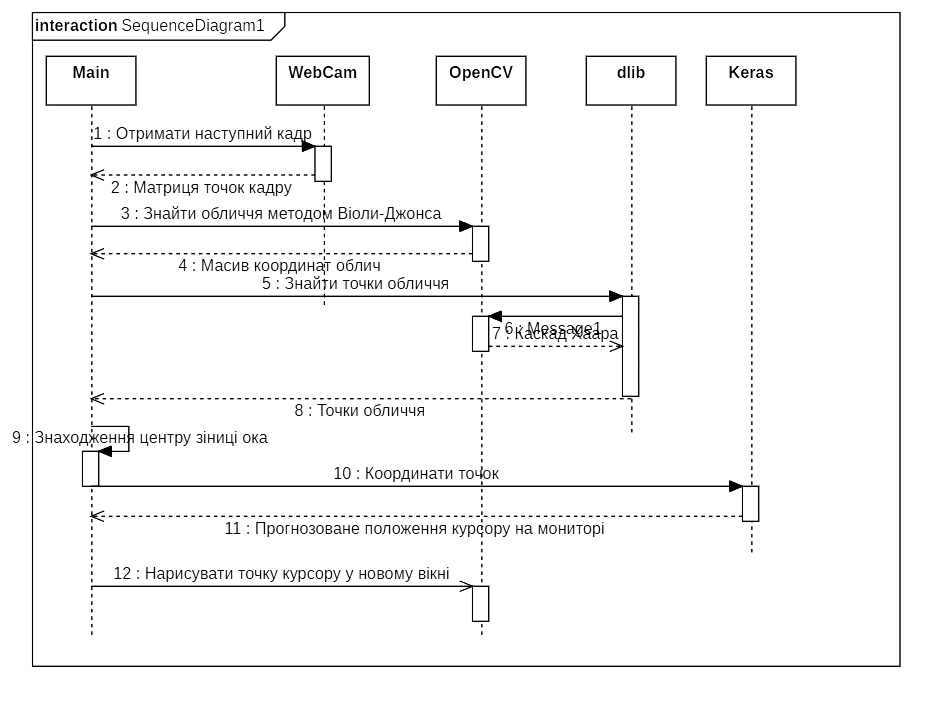
\includegraphics[width=\textwidth]{uml_sequence}
	\caption{UML-діаграма послідовності}
	\label{fig:sequence}
\end{figure} 

\subsubsection{Схема нейронної мережі}
На рисунку~\ref{fig:network} зображена схема нейронної мережі.

\begin{figure}[H]
	\centering
	\includegraphics[width=\textwidth]{network}
	\caption{Схема нейронної мережі}
	\label{fig:network}
\end{figure} 

Нейронна мережа буде складатися з п'яти шарів:
\begin{enumerate}[label={\arabic*-й ---}]
	\item має форму $256\times2$ та лінійну функцію активації; 
	\item має форму $128\times2$ та лінійну функцію активації; 
	\item має форму $64\times2$ та лінійну функцію активації; 
	\item має форму $256\times1$ та функцію активації сігмоїда; 
	\item має форму $2\times1$ та функцію активації сігмоїда. 
\end{enumerate}

На вхід подається матриця нормалізованих координат специфічних точок обличчя, які зображені на рисунку~\ref{fig:face}. 

\begin{figure}[H]
	\centering
	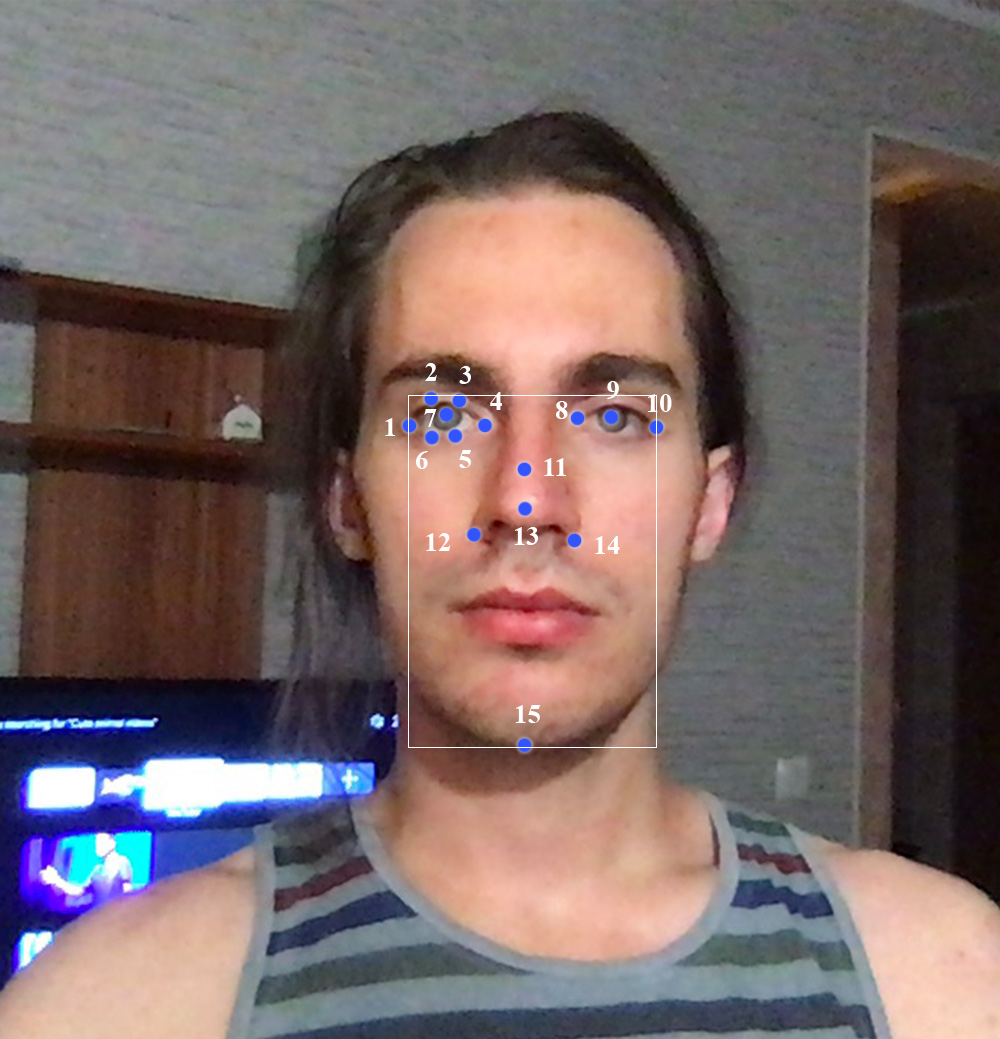
\includegraphics[width=0.6\textwidth]{face}
	\caption{Точки, які використовуються для визначення погляду}
	\label{fig:face}
\end{figure} 

Додаткові точки на правому оці використовуються для розпізнавання блимків, які транслюються у кликі мишою.

\subsection{Обґрунтування вибору платформи розробки та інструментальних засобів}
\subsubsection{Мова програмування Python}
Python чудово підходить для вирішення задач машинного навчання, дозволяя писати стислий та експресивний код.

\subsubsection{Система управління версіями Git}
Використання системи контролю версії є необхідним для роботи над великими проектами.

Система контролю дозволяє зберігати попередні версії файлів та завантажувати їх за потребою. 
Вона зберігає повну інформацію про версію кожного з файлів, а також повну структуру проекту на всіх стадіях розробки.

Git --- розподілена система керування версіями файлів та спільної роботи. Git є однією з найефективніших, надійних і високопродуктивних систем керування версіями, що надає гнучкі засоби нелінійної розробки, що базуються на відгалуженні і злитті гілок.

\subsubsection{Середовище розробки застосунків Visual Code}
Visual Code --- швидкий кросплатформенний редактор вихідних текстів програм. Підтримує плагіни для розробки за допомогою мови програмування Python.
